% ============================================================
% Market Deformation Geometry
% A Teichmüller-Geometric Framework for Multi-Asset and
% Multi-Broker Market Analysis
%
% This file is the CANONICAL SOURCE of the paper; the PDF is
% built from it. Build: pdflatex (twice, for TOC/refs).
% ============================================================

\documentclass[11pt,a4paper]{article}

\usepackage[T1]{fontenc}
\usepackage[utf8]{inputenc}
\usepackage{lmodern}
\usepackage{microtype}
\usepackage[margin=2.5cm]{geometry}

\usepackage{amsmath,amssymb,amsthm,mathtools,bm}
\usepackage{mathrsfs}
\usepackage{booktabs,array,longtable}
\usepackage{enumitem}
\usepackage{graphicx}
\usepackage{xcolor}
\usepackage{tikz}
\usetikzlibrary{arrows.meta,positioning,calc}
\usepackage{verbatim}

\usepackage{hyperref}
\hypersetup{
  colorlinks=true,
  linkcolor=blue!50!black,
  citecolor=blue!50!black,
  urlcolor=blue!50!black,
  pdftitle={Market Deformation Geometry: A Teichmüller Framework
            for Structural Change Detection in Multi-Asset,
            Multi-Venue Markets},
  pdfauthor={Marc Brendecke},
  pdfkeywords={Teichmuller theory, quasiconformal mappings,
               Beltrami coefficient, structural change detection,
               regime detection, market microstructure,
               multi-venue, multi-asset, foreign exchange}
}

\usepackage{fancyhdr}
\pagestyle{fancy}
\fancyhf{}
\lhead{Market Deformation Geometry}
\rhead{\thepage}
\renewcommand{\headrulewidth}{0.4pt}

\numberwithin{equation}{section}

% ------------------------------------------------------------
% Theorem environments
% ------------------------------------------------------------

\newtheorem{definition}{Definition}[section]
\newtheorem{hypothesis}{Hypothesis}
\newtheorem{remark}{Remark}[section]

% ------------------------------------------------------------
% Mathematical commands
% ------------------------------------------------------------

\newcommand{\R}{\mathbb{R}}
\newcommand{\C}{\mathbb{C}}
\newcommand{\E}{\mathbb{E}}
\newcommand{\Var}{\operatorname{Var}}
\newcommand{\Cov}{\operatorname{Cov}}
\newcommand{\tr}{\operatorname{tr}}
\newcommand{\med}{\operatorname{median}}
\newcommand{\argmin}{\operatorname*{arg\,min}}
\newcommand{\abs}[1]{\left|#1\right|}
\newcommand{\norm}[1]{\left\lVert#1\right\rVert}
\newcommand{\inner}[2]{\left\langle#1,#2\right\rangle}

\newcommand{\Tgrid}{\mathcal{T}}
\newcommand{\Aset}{\mathcal{A}}
\newcommand{\Bset}{\mathcal{B}}
\newcommand{\Cset}{\mathcal{C}}
\newcommand{\Tmkt}{\mathcal{T}_{\mathrm{mkt}}}
\newcommand{\Xspace}{\mathcal{X}}

% ============================================================
\title{
\textbf{Market Deformation Geometry}
\\[0.5em]
\large
A Teichmüller Framework for Structural Change Detection\\
in Multi-Asset, Multi-Venue Markets
}

\author{Marc Brendecke\\[0.15em]\small Independent Research}

\date{August 2026}

% ============================================================
\begin{document}

\maketitle

\begin{abstract}
This paper proposes \emph{Market Deformation Geometry}: a
structure-first Teichmüller framework that measures structural
change in multi-asset, multi-venue financial markets as
quasiconformal deformation of synchronized price observations. The
observable market is represented not as a collection of isolated
price charts, but as a coupled multidimensional geometric object.
Foreign exchange serves
as the running example throughout, because it supplies many
algebraically related instruments and multiple observable price
feeds; the construction itself applies to any universe of
instruments observed through several venues.

The fundamental data structure is the synchronized tensor
$P(t,a,b)$, where $t$ denotes time, $a$ an asset --- a currency
pair, a metal, an index, or any other instrument --- and $b$ a
broker or price-feed observation. The temporal coordinate describes
the evolution of the market, the asset coordinate describes
cross-asset relationships, and the broker coordinate describes
different realizations of nominally identical market instruments.

The central observation is that these dimensions must not be treated
as interchangeable. Connecting observations along the time axis
produces a conventional price path. Connecting observations along
the broker axis instead produces a cross-sectional observation
geometry. Connecting assets produces a third structural direction.
The paper develops finite-difference analogues of
$\partial_tP$, $\partial_aP$, $\partial_bP$ together with the mixed
derivatives $\partial_t\partial_aP$, $\partial_t\partial_bP$,
$\partial_a\partial_bP$. Particular attention is given to
$\partial_t\partial_bP$, which measures how the temporal evolution
of an instrument differs across broker observations.

The second part of the framework introduces a quasiconformal
geometric layer. Local market patches are normalized and compared by
deformation maps; the Beltrami coefficient
$\mu=f_{\bar z}/f_z$ and the quasiconformal dilatation
$K=(1+\abs{\mu})/(1-\abs{\mu})$ provide candidate measures of
structural deformation. The proposed financial interpretation is
deliberately conservative: the market is not assumed to literally be
a Riemann surface. Instead, market data are embedded into
finite-dimensional geometric patches, and quasiconformal mappings
are used as a mathematical comparison device.

The literature already contains geometric approaches to finance ---
manifold learning, Riemannian and Minkowski formulations,
topological and cohomological constructions, and a direct use of
Teichmüller and moduli-space ideas in financial time-series
classification. The proposed contribution is therefore not
``geometry in finance'' in general; the specific gap addressed is
the \emph{combination} of synchronized multi-asset observations,
multiple observation venues, explicit quasiconformal deformation,
and a Teichmüller-type market distance.

The resulting framework defines a market state in terms of
geometric deformation, cross-asset coherence, cross-broker
coherence, mixed-dimensional coupling, and triangular consistency,
and formulates empirical hypotheses, null models, estimator
validation, falsification tests, and potential applications to
regime detection. A statistical-power pre-calculation determines
which hypotheses the planned dataset can decide: window-level
coherence hypotheses within the first cycle, event-level transition
hypotheses only for large effects, and economic significance not at
all on realistic horizons. A first implementation cycle sharpens
both the mathematics and the empirics: on simply connected patches
the proposed distance is identically zero by the Riemann mapping
theorem, and the tractable carrier of Teichmüller structure is the
torus, where the distance acquires a closed form on conformal
classes of $2\times2$ covariances and coordinate robustness (H7)
becomes a theorem for that estimator; empirically, the venue axis
fails as a geometric direction but serves as a replication axis,
giving the conformal shape a measured error floor roughly a factor
of ten below its movement through time. The primary research question is not whether a
new indicator can be invented, but whether the multidimensional
geometry of synchronized market observations contains information
that cannot be reduced to volatility, correlation, PCA,
cointegration, or standard technical indicators.
\end{abstract}

\tableofcontents

\newpage

% ============================================================
\section{Introduction}
% ============================================================

Conventional financial chart analysis begins with a one-dimensional
time series $P(t)$. The independent variable is time and the
dependent variable is price. From this representation one constructs
moving averages, oscillators, volatility estimators, channels, trend
lines, and other derived statistics.

This representation is useful, but it removes information that is
intrinsic to real markets. Foreign exchange makes the loss
especially visible and serves as the running example; the
construction is not restricted to it
(Section~\ref{sec:generalization}).

A currency pair is not an isolated object. It is related to other
currency pairs through currency identities, triangular
relationships, liquidity conditions, funding relationships, order
flow, and market microstructure. A metal, an index, or a
crypto-asset is likewise coupled to the rest of the universe ---
through common risk factors, funding currencies, and shared
liquidity --- even where no exact algebraic identity exists.

Furthermore, the same nominal instrument can be observed through
multiple brokers or liquidity sources. These observations are
similar but generally not identical.

Consequently, instead of considering only $P(t)$, we propose the
multidimensional object
\[
\boxed{P(t,a,b)}
\]
with
\[
t:\text{ time},\qquad
a:\text{ asset / instrument},\qquad
b:\text{ broker / observation source}.
\]

This creates three distinct directions. For fixed $(a,b)$, the map
$t\mapsto P(t,a,b)$ is the conventional price chart. For fixed
$(t,a)$, the map $b\mapsto P(t,a,b)$ describes the cross-broker
realization of the same instrument at the same moment. For fixed
$(t,b)$, the map $a\mapsto P(t,a,b)$ describes the cross-asset
market state.

The complete object therefore contains substantially more structure
than an ordinary chart. The main proposition of this paper is:

\begin{quote}
The geometry of the multidimensional observation structure may
contain information about market regimes that is not visible in an
individual price path.
\end{quote}

The proposed framework is deliberately structure-first. No trading
rule is assumed in advance. The research sequence is
\[
\text{market data}
\rightarrow
\text{geometric representation}
\rightarrow
\text{deformation}
\rightarrow
\text{market state}
\rightarrow
\text{empirical validation}.
\]

% ============================================================
\section{Related Work and the Research Gap}\label{sec:related}
% ============================================================

Geometric approaches to finance are established, and the present
framework must be positioned against them rather than beside them.
Differential-geometric methods have long been used in asset pricing
and incomplete-market models, while more recent work embeds
financial observations into low-dimensional manifolds. A directly
relevant recent example is the use of constant-curvature
two-manifolds as latent geometries for financial data, with
spherical, Euclidean, hyperbolic, and toroidal candidates compared
empirically \cite{Papaioannou2025}. Pinčák and Kanjamapornkul
explicitly couple price and time through a Minkowski metric in a
GARCH framework \cite{PincakKanjamapornkul2018}, and a cohomological
and topological treatment of financial time series --- including
link and knot structures and a topological interpretation of
bid--ask dynamics --- has also been proposed
\cite{Kanjamapornkul2020}.

The closest direct prior art identified is the \emph{Support Spinor
Machine} \cite{Kanjamapornkul2017}, which uses moduli-space and
Teichmüller-space ideas as part of a nonlinear time-series
classification architecture. It would therefore be incorrect to
claim that Teichmüller concepts have never been applied to financial
time series. The claim of this paper is narrower. The intended
research gap is
\[
\boxed{
\begin{gathered}
\text{synchronized multi-asset observations}
\times
\text{multiple venues}\\
\times\;
\text{explicit quasiconformal deformation}
\times
\text{Teichmüller-type market distance}
\end{gathered}
}
\]
--- that is, the specific combination, not any individual
ingredient.

Two further strands border the empirical part of this paper, and
the boundary should be drawn precisely. First, multi-venue
econometrics treats the dispersion between venues as a nuisance:
fragmentation noise to be modeled and removed so that integrated
variance can be estimated consistently \cite{DiasSchweikert2026}.
The present framework inverts that stance --- venue dispersion is
retained as a replicate-based error bar for geometric statistics
(Section~\ref{sec:firstcycle}); the analytic null distribution for
geodesic distances between correlation matrices
\cite{Kuketayev2026}, built on the quotient-affine geometry of
\cite{ThanwerdasPennec2021}, is the model-based complement to such
a measured floor, not a substitute for it. Second, the slow
evolution of market correlation structure is an established
econophysics finding: correlation-matrix similarity defines
persistent market states \cite{Muennix2012}, and the correlation
structure of U.S.\ industry indices evolves on well-separated
time scales --- the average correlation on a scale beyond five
years, the leading spectral quantities in event-driven bursts
\cite{BuccheriMarmiMantegna2013}. That phenomenon is not claimed
as new here; what this paper adds on that front is the
instrument --- a scale- and $\mathrm{GL}(2)$-invariant distance
with a closed form and a proof of extremality, reported together
with its measured error floor.

Classical quasiconformal and Teichmüller theory provides the
mathematical foundation; the standard modern framework is Gardiner
and Lakic \cite{GardinerLakic2000}, with \cite{Ahlfors1966} and
\cite{AstalaIwaniecMartin} as classical references. In local complex
coordinates, a quasiconformal map satisfies
\begin{equation}
f_{\bar z}=\mu(z)\,f_z,\qquad\norm{\mu}_\infty<1,
\end{equation}
with the local distortion $K(z)$ developed in
Section~\ref{sec:qc}.

To keep the boundary between foundation and proposal visible, every
construction in this paper is assigned one of three statuses ---
\emph{established mathematics}, \emph{proposed construction}, or
\emph{research hypothesis} --- and Appendix~\ref{app:status} records
this assignment per component.

% ============================================================
\section{The Market Tensor \texorpdfstring{$P(t,a,b)$}{P(t,a,b)}}
% ============================================================

Let $\Tgrid=\{t_1,\ldots,t_T\}$ be a common time grid, let
$\Aset=\{a_1,\ldots,a_N\}$ be the set of instruments --- in the FX
example currency pairs, in general any mix of asset classes --- and
let $\Bset=\{b_1,\ldots,b_M\}$ be the set of brokers or independent
price-feed sources.

The synchronized price tensor is defined as
\begin{equation}
P_{ijk}=P(t_i,a_j,b_k).
\label{eq:market_tensor}
\end{equation}
Thus the complete data structure has $T\times N\times M$ price
observations before considering bid, ask, OHLC, volume, spread, or
order-book information.

\begin{definition}[Market Tensor]
The synchronized market tensor is
\[
\Xspace=
\left\{
P(t,a,b)\;\middle|\;
t\in\Tgrid,\ a\in\Aset,\ b\in\Bset
\right\}.
\]
\end{definition}

The tensor should be interpreted as an observation structure rather
than as a conventional three-dimensional physical space. The
coordinates have different meanings; $(t,a,b)$ is therefore
\emph{not} symmetric under arbitrary coordinate permutations.

% ============================================================
\section{Temporal Synchronization of Multi-Venue Data}
% ============================================================

Cross-broker comparison requires a common temporal coordinate.
Suppose broker $b_1$ constructs a five-minute bar over
$[12{:}00,12{:}05)$ while broker $b_2$ constructs a bar over
$[12{:}01,12{:}06)$. The resulting bars cannot be compared directly
without introducing an artificial phase displacement.

We therefore define a canonical partition
$\mathcal{I}=\{I_1,\ldots,I_T\}$ and a synchronization operator
\[
\mathscr{S}:P^{(b)}\mapsto P^{(b)}_{\mathcal{I}}.
\]
All brokers must be mapped onto the same canonical intervals.

For tick data, the synchronization problem is more subtle because
quotes arrive asynchronously. Possible approaches include:
\begin{enumerate}
\item previous-tick interpolation;
\item linear interpolation;
\item event-time sampling;
\item nearest-neighbor synchronization;
\item volume-clock or transaction-clock synchronization.
\end{enumerate}
The chosen procedure must be fixed before statistical testing.

% ============================================================
\section{Logarithmic Price Coordinates}
% ============================================================

Prices are multiplicative quantities. Define
\begin{equation}
x(t,a,b)=\log P(t,a,b).
\label{eq:logprice}
\end{equation}
The temporal return becomes
\begin{equation}
r_t(t,a,b)=x(t+\Delta t,a,b)-x(t,a,b).
\label{eq:return}
\end{equation}

Logarithmic coordinates are particularly useful because cross-rate
relationships become additive. For example,
$\mathrm{EUR/JPY}=(\mathrm{EUR/USD})(\mathrm{USD/JPY})$ implies
\[
\log(\mathrm{EUR/JPY})
=\log(\mathrm{EUR/USD})+\log(\mathrm{USD/JPY}).
\]
This provides a natural connection between the asset dimension and
the underlying currency dimension.

% ============================================================
\section{Currency-Network Representation}
% ============================================================

This section and the two that follow exploit relational structure
that is specific to currencies. In a broader universe they apply to
the FX subgraph; instruments without exact algebraic
cross-identities simply contribute no closure constraints, while the
temporal and broker dimensions apply to them unchanged.

Let $\Cset=\{c_1,\ldots,c_K\}$ denote the currency universe. An FX
pair $i/j$ can be represented through latent currency coordinates
$u_i(t,b)$ and $u_j(t,b)$. Define
\begin{equation}
x_{ij}(t,b)=u_i(t,b)-u_j(t,b)+\varepsilon_{ij}(t,b).
\label{eq:currency_factor}
\end{equation}
The residual $\varepsilon_{ij}$ contains quotation noise,
microstructure effects, timing effects, and deviations from the
latent currency representation.

The representation has a gauge freedom because
$(u_i+\lambda)-(u_j+\lambda)=u_i-u_j$. We therefore impose
\begin{equation}
\sum_{i=1}^{K}u_i(t,b)=0.
\label{eq:gauge}
\end{equation}
This converts the currency system into a normalized coordinate
system.

% ============================================================
\section{The Currency Graph and Its Incidence Matrix}
% ============================================================

Let $G_A=(V_A,E_A)$ be the directed currency graph. Currencies form
vertices, $V_A=\Cset$; FX pairs form directed edges,
$E_A\subseteq\Cset\times\Cset$.

Let $B$ denote the incidence matrix. Then the vector of pairwise log
prices may be approximated by
\begin{equation}
\bm{x}(t,b)=B\bm{u}(t,b)+\bm{\varepsilon}(t,b).
\label{eq:graph_model}
\end{equation}
This representation is useful because it allows the cross-asset
layer to be interpreted as a projection of a smaller currency state.

% ============================================================
\section{Triangular No-Arbitrage Consistency}
% ============================================================

For three currencies $i,j,k$, the identity
$x_{ij}+x_{jk}+x_{ki}=0$ holds in the idealized frictionless case.
Define the triangular residual
\begin{equation}
\tau_{ijk}(t,b)=x_{ij}(t,b)+x_{jk}(t,b)+x_{ki}(t,b).
\label{eq:triangle}
\end{equation}
In real markets $\tau_{ijk}\neq0$ because of spreads, transaction
costs, latency, quotation conventions, and liquidity constraints.
The residual should therefore be treated as a structural observable,
not as an automatic arbitrage signal.

Exact closure identities of this kind are a privilege of the
currency subgraph. Other asset classes contribute analogous but
weaker consistency relations --- the spot--futures basis of a metal
or index, or the cross-venue identity of the same crypto-asset ---
and where no such relation exists, the venue dimension alone
supplies the consistency structure: the same instrument observed
twice must agree up to the broker operators of
Section~\ref{sec:brokerops}.

% ============================================================
\section{The Three Geometric Directions: Time, Asset, Broker}
% ============================================================

The market tensor possesses three fundamental directional
variations.

\subsection{Temporal direction}

The discrete temporal derivative is
\begin{equation}
\Delta_tP_{ijk}=P_{i+1,j,k}-P_{i,j,k}.
\label{eq:dt}
\end{equation}
This is the ordinary direction of chart movement.

\subsection{Asset direction}

For appropriately normalized asset coordinates,
\begin{equation}
\Delta_aP_{ijk}=P_{i,j+1,k}-P_{i,j,k}.
\label{eq:da}
\end{equation}
This represents cross-asset structural variation. Because arbitrary
numerical ordering of assets is generally meaningless, a practical
implementation should preferably replace the raw index $j$ with a
graph, factor, or manifold coordinate.

\subsection{Broker direction}

For fixed time and asset,
\begin{equation}
\Delta_bP_{ijk}=P_{i,j,k+1}-P_{i,j,k}.
\label{eq:db}
\end{equation}
This is the crucial observation dimension. It is not another time
series. It represents the dispersion of nominally identical market
observations. The ordering caveat of the asset direction applies
here with full force: venue indices carry no canonical order, so
any statistic built on $\Delta_bP$ must be symmetrized --- in
practice through pairwise differences
(Section~\ref{sec:firstcycle}).

% ============================================================
\section{The Broker Fiber: Cross-Venue Price Dispersion}
% ============================================================

For fixed $(t,a)$ define the broker fiber
\begin{equation}
\mathcal{F}_{t,a}=\left\{P(t,a,b):b\in\Bset\right\}.
\end{equation}
A robust central observation is
\begin{equation}
\bar{x}(t,a)=\med_b\,x(t,a,b).
\label{eq:broker_median}
\end{equation}
The broker deviation is
\begin{equation}
d_b(t,a,b)=x(t,a,b)-\bar{x}(t,a).
\label{eq:broker_deviation}
\end{equation}
A robust dispersion measure is
\begin{equation}
\sigma_b(t,a)=1.4826\,\med_b\abs{d_b(t,a,b)}.
\label{eq:broker_mad}
\end{equation}
The coefficient $1.4826$ converts the MAD to the standard-deviation
scale under Gaussian assumptions.

% ============================================================
\section{Mixed Temporal--Broker Geometry}
% ============================================================

The most important broker statistic is not simply $\Delta_bP$.
Instead, consider its temporal evolution. Define
\begin{equation}
\Delta_t\Delta_bP_{ijk}
=\left(P_{i+1,j,k+1}-P_{i+1,j,k}\right)
-\left(P_{i,j,k+1}-P_{i,j,k}\right).
\label{eq:dt_db}
\end{equation}
In continuous notation, $\partial_t\partial_bP$. This quantity
answers:
\begin{quote}
Do two broker observations evolve differently during the same market
movement?
\end{quote}

A small broker spread that remains structurally stable may be
uninteresting. A rapidly changing broker differential may indicate:
\begin{itemize}
\item liquidity fragmentation;
\item feed latency;
\item different liquidity providers;
\item spread expansion;
\item asynchronous quote updates;
\item market microstructure stress;
\item timestamp problems.
\end{itemize}

% ============================================================
\section{Cross-Asset Temporal Geometry}
% ============================================================

Analogously, $\Delta_t\Delta_aP$ measures how temporal movement
differs across assets. This is fundamentally different from simple
correlation.

Correlation asks: \emph{do two return series move together?} The
mixed derivative asks: \emph{how does the local temporal geometry
vary across the asset dimension?}

The distinction becomes important during transitions. Two assets may
retain high correlation while their local geometric structure
changes dramatically.

% ============================================================
\section{First- and Second-Order Differential Structure}
% ============================================================

The differential of the market field is formally
\begin{equation}
dP=P_t\,dt+P_a\,da+P_b\,db.
\label{eq:dP}
\end{equation}
The second-order differential contains
\begin{equation}
\begin{aligned}
d^2P={}&P_{tt}\,dt^2+P_{aa}\,da^2+P_{bb}\,db^2\\
&+2P_{ta}\,dt\,da+2P_{tb}\,dt\,db+2P_{ab}\,da\,db.
\end{aligned}
\label{eq:d2P}
\end{equation}
The six second-order components have different interpretations.
$P_{tt}$ describes temporal curvature; $P_{aa}$ describes curvature
across assets; $P_{bb}$ describes curvature across broker
observations. The mixed components $P_{ta}$, $P_{tb}$, $P_{ab}$
describe interactions between the three market dimensions.

% ============================================================
\section{Local Market Surfaces and the Induced Metric}
% ============================================================

Fix an asset $a$ and define a broker-time surface
\begin{equation}
S_a(t,b)=x(t,a,b).
\label{eq:broker_surface}
\end{equation}
The local tangent vectors are $S_t=\partial_tS$ and
$S_b=\partial_bS$. The induced metric is
\begin{equation}
g=
\begin{pmatrix}
\inner{S_t}{S_t}&\inner{S_t}{S_b}\\
\inner{S_b}{S_t}&\inner{S_b}{S_b}
\end{pmatrix}.
\label{eq:metric}
\end{equation}
Define
\begin{equation}
\rho_{tb}=\frac{g_{tb}}{\sqrt{g_{tt}g_{bb}}}.
\label{eq:rho_tb}
\end{equation}
This is a normalized local coupling between temporal and broker
variation. Similarly, for fixed broker $b$, the surface
$S_b(t,a)=x(t,a,b)$ produces an asset-time surface, and
\begin{equation}
\rho_{ta}=\frac{g_{ta}}{\sqrt{g_{tt}g_{aa}}}
\label{eq:rho_ta}
\end{equation}
measures temporal-asset coupling.

% ============================================================
\section{The Tensor as a Family of Coupled Surfaces}
% ============================================================

The three surfaces $(t,a)$, $(t,b)$, and $(a,b)$ are projections of
the same underlying tensor.

\begin{center}
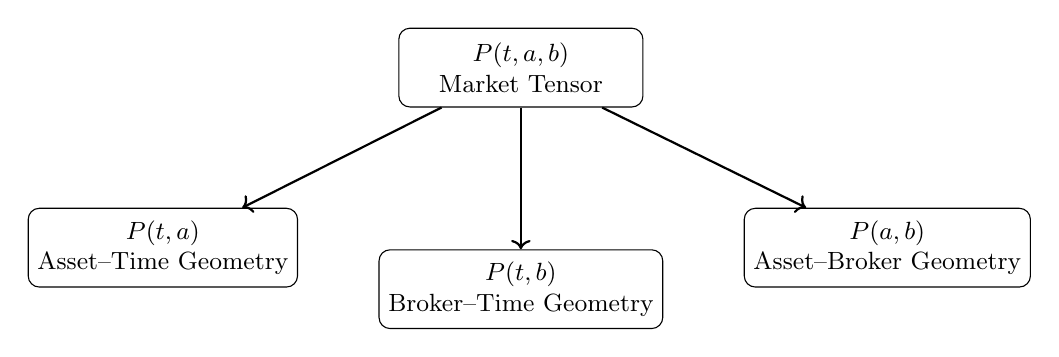
\begin{tikzpicture}[
    node distance=1.8cm,
    every node/.style={font=\small},
    box/.style={
        draw,rounded corners,
        minimum width=3.1cm,minimum height=1cm,align=center
    }
]
\node[box] (tensor) {$P(t,a,b)$\\Market Tensor};
\node[box,below left=of tensor] (timeasset)
  {$P(t,a)$\\Asset--Time Geometry};
\node[box,below=of tensor] (timebroker)
  {$P(t,b)$\\Broker--Time Geometry};
\node[box,below right=of tensor] (assetbroker)
  {$P(a,b)$\\Asset--Broker Geometry};
\draw[->,thick] (tensor) -- (timeasset);
\draw[->,thick] (tensor) -- (timebroker);
\draw[->,thick] (tensor) -- (assetbroker);
\end{tikzpicture}
\end{center}

The complete market geometry should therefore be regarded as a
family of coupled surfaces rather than as a single chart.

% ============================================================
\section{Quasiconformal Maps and the Beltrami Coefficient}\label{sec:qc}
% ============================================================

A central question is how one local market geometry changes into
another. Let $\Phi_0$ be a reference market patch and $\Phi_1$ a
later market patch. We seek a map
\begin{equation}
f:\Phi_0\rightarrow\Phi_1.
\end{equation}
For a complex coordinate $z=x+iy$, a sufficiently regular map can be
written locally as $df=f_z\,dz+f_{\bar z}\,d\bar z$. The Beltrami
coefficient is
\begin{equation}
\mu(z)=\frac{f_{\bar z}(z)}{f_z(z)}.
\label{eq:beltrami}
\end{equation}
For an orientation-preserving quasiconformal map, $\abs{\mu(z)}<1$.
The local dilatation is
\begin{equation}
K(z)=\frac{1+\abs{\mu(z)}}{1-\abs{\mu(z)}}.
\label{eq:dilatation}
\end{equation}
When $\mu=0$ the transformation is locally conformal and $K=1$. As
$\abs{\mu}\rightarrow1$, the distortion increases.

% ============================================================
\section{Financial Interpretation of the Beltrami Field}
\label{sec:beltrami-interp}
% ============================================================

The proposed interpretation is
\[
\boxed{\mu\quad\leftrightarrow\quad\text{local market deformation}}
\]
and
\[
\boxed{K\quad\leftrightarrow\quad
\text{magnitude of structural distortion}.}
\]

This interpretation must be treated as a modeling construction. It
is \emph{not} claimed that the observed market is intrinsically a
complex manifold. Instead, the financial data are embedded into a
local two-dimensional coordinate patch.

One possible coordinate system is $z=u+iv$ with $u$ a normalized
time and $v$ a normalized cross-sectional coordinate. The
cross-sectional coordinate may represent:
\begin{enumerate}
\item broker rank;
\item a latent currency factor;
\item a PCA coordinate;
\item a diffusion-map coordinate;
\item a graph coordinate.
\end{enumerate}

% ============================================================
\section{A Teichmüller-Type Deformation Distance}
% ============================================================

Let $\Phi_0,\Phi_1$ be normalized market patches. Define the minimal
quasiconformal distortion
\begin{equation}
K_{\min}=\inf_f\sup_zK_f(z),
\label{eq:kmin}
\end{equation}
where $f$ ranges over the admissible deformation maps. We then
define the proposed geometric distance
\begin{equation}
D_T(\Phi_0,\Phi_1)=\frac12\log K_{\min}.
\label{eq:teich_distance}
\end{equation}
This is inspired by the standard logarithmic quasiconformal metric
structure of Teichmüller theory. The financial quantity should
therefore be interpreted as a \emph{Teichmüller-inspired deformation
statistic}.

\subsection{Degeneracy on simply connected patches}
\label{sec:degeneracy}

The definition above has a failure mode that is easy to miss and
fatal if missed. If two market patches are simply connected plane
domains without marked points, the Riemann mapping theorem supplies
a \emph{conformal} map between them, hence $K_{\min}=1$ and
$D_T\equiv0$ --- for every pair of market states. Whatever a
general-purpose implementation reports as nonzero on such patches
is a property of its own normalization, not of the market. A
nontrivial Teichmüller distance requires actual moduli: marked
points, or nontrivial topology.

\subsection{The torus: an exact, closed-form carrier}
\label{sec:torus}

Exactly one tractable carrier is available in this setting. A flat
metric on the torus is a positive-definite $2\times2$ matrix; its
conformal class is that matrix modulo a positive scale factor; and
$\mathrm{SPD}(2)/\mathbb{R}_{+}$ \emph{is} the Teichmüller space of
the torus. The extremal map between flat tori is affine
(Teichmüller's theorem; the quadratic differential is $dz^2$), so
the inf--sup in \eqref{eq:kmin} has a closed solution. With
$\Sigma_1,\Sigma_2$ the shape matrices normalized to determinant
one, $\Lambda=\Sigma_1^{-1}\Sigma_2$, $T=\operatorname{tr}\Lambda$,
and $\lambda_{+}=\bigl(T+\sqrt{T^2-4}\bigr)/2$,
\begin{equation}
d_T=\tfrac12\log\lambda_{+}.
\label{eq:torusdist}
\end{equation}
Up to a constant factor this is the affine-invariant metric on
covariance matrices. The Teichmüller provenance does not supply a
new number --- it supplies the \emph{proof that this number is the
extremal one}, and it removes the optimization that Stage~IV of the
research programme otherwise requires on two-dimensional patches.

What \eqref{eq:torusdist} buys beyond a correlation is precisely
one property: $d_T$ is invariant under $\mathrm{GL}(2)$ changes of
basis of the plane (modulo scale), whereas the PCA concentration
$\lambda_1/\operatorname{tr}\Sigma$ is not. For this estimator,
coordinate robustness (H7) is therefore a theorem rather than a
hypothesis; the hypothesis remains open for every other estimator
in this paper. Two boundaries stay in force:
$\mathrm{GL}(2)$-invariance protects against coordinates
\emph{within} the plane, not against the choice of the plane
itself, which must be preregistered; and the identification is
exact only in dimension two --- for larger universes the
affine-invariant geometry of $\mathrm{SPD}(N)$ remains available,
but should then be called by that name.

% ============================================================
\section{Market Teichmüller Space}\label{sec:teichspace}
% ============================================================

Let $\mathfrak{M}$ denote the set of normalized market patches.
Introduce an equivalence relation $\Phi_1\sim\Phi_2$ when the two
patches differ only through the chosen admissible normalizations and
conformal transformations. The resulting quotient is denoted
\begin{equation}
\Tmkt=\mathfrak{M}/\sim.
\label{eq:market_teich}
\end{equation}
A market state becomes $[\Phi_t]\in\Tmkt$, and a market trajectory
is $t\mapsto[\Phi_t]$. The corresponding geometric velocity is
\begin{equation}
V_G(t)=\frac{D_T(\Phi_t,\Phi_{t+\Delta t})}{\Delta t}.
\label{eq:geovelocity}
\end{equation}
The geometric acceleration is
\begin{equation}
A_G(t)=V_G(t)-V_G(t-\Delta t).
\label{eq:geoacceleration}
\end{equation}

% ============================================================
\section{Price Movement versus Structural Movement}
% ============================================================

A geometrically stable market regime satisfies approximately
$D_T(\Phi_t,\Phi_{t+\Delta t})\approx0$. A transition satisfies
$D_T(\Phi_t,\Phi_{t+\Delta t})\uparrow$. A rapidly developing
structural transition satisfies $A_G(t)\gg0$.

This gives a conceptual distinction between price movement and
structural movement. A market may exhibit $\abs{\Delta P}\gg0$ while
$D_T\approx0$. This would correspond to a strong movement that
preserves the local market geometry.

Conversely, $\abs{\Delta P}\approx0$ may coexist with $D_T\gg0$.
This would indicate a structural transition occurring before a
large-amplitude price movement.

% ============================================================
\section{Cross-Broker Coherence}
% ============================================================

Define broker return dispersion
\begin{equation}
\sigma_B^2(t,a)=\Var_b\left[r_t(t,a,b)\right].
\end{equation}
A normalized coherence statistic may be defined as
\begin{equation}
C_B(t,a)=1-\frac{\sigma_B(t,a)}{\sigma_{\mathrm{ref}}(t,a)+\epsilon}.
\label{eq:CB}
\end{equation}
The precise bounded normalization should be chosen empirically. A
high value indicates that the temporal realization of the same
instrument is similar across brokers; a low value indicates
divergence.

% ============================================================
\section{Cross-Asset Coherence}
% ============================================================

Let $\bm{r}_t$ be the vector of normalized asset returns and let
$\Sigma_t=\Cov(\bm{r}_t)$ be the local covariance matrix. The first
principal component explains
\begin{equation}
C_A(t)=\frac{\lambda_1(\Sigma_t)}{\tr(\Sigma_t)}.
\label{eq:CA}
\end{equation}
This is a benchmark measure of cross-asset coherence. The proposed
geometric framework should be tested \emph{against} this quantity
rather than simply replacing it.

% ============================================================
\section{Joint Market Coherence}
% ============================================================

A simple composite statistic is
\begin{equation}
C_{AB}(t)=C_A(t)C_B(t).
\label{eq:CAB}
\end{equation}
A more rigorous implementation would estimate a joint latent
coherence factor. The conceptual interpretation is that
$C_{AB}\approx1$ means the market is coherent across both assets and
broker observations.

% ============================================================
\section{The Geometric Market State Vector}
% ============================================================

Define the state vector
\begin{equation}
\mathbf{S}_t=
\begin{pmatrix}
D_T(t)&V_G(t)&A_G(t)&C_A(t)&C_B(t)&D_{ta}(t)&D_{tb}(t)&\tau(t)
\end{pmatrix}^{\!\top}.
\label{eq:state_vector}
\end{equation}
This vector is the central candidate representation of market state.
It deliberately avoids reducing the market to a single scalar.

% ============================================================
\section{The Coherence--Deformation Phase Diagram}
% ============================================================

A particularly useful projection is $x=C_{AB}$ against $y=D_T$. This
produces the qualitative phase structure below.

\begin{center}
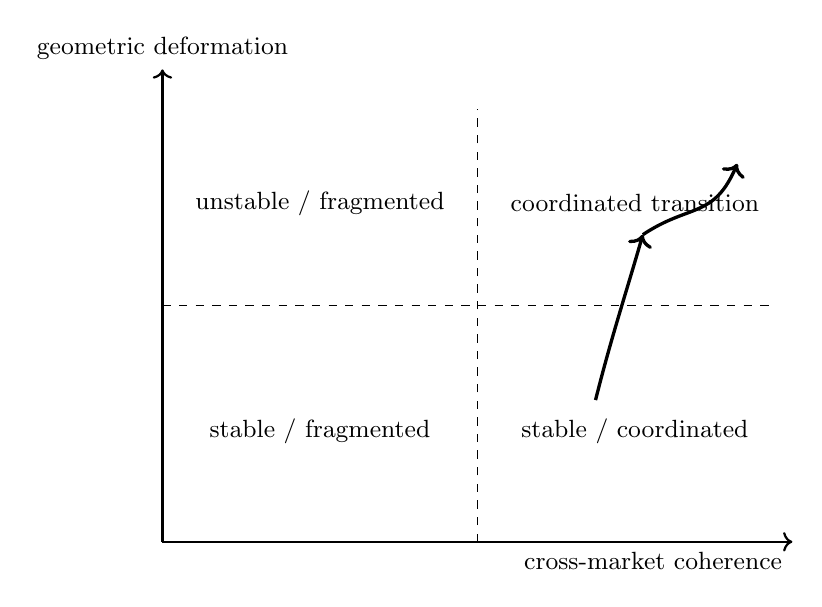
\begin{tikzpicture}[scale=1.0]
\draw[->,thick] (0,0) -- (8,0)
    node[below left,font=\small] {cross-market coherence};
\draw[->,thick] (0,0) -- (0,6)
    node[above,font=\small] {geometric deformation};
\draw[dashed] (4,0) -- (4,5.5);
\draw[dashed] (0,3) -- (7.7,3);
\node[font=\small] at (2,1.4) {stable / fragmented};
\node[font=\small] at (6,1.4) {stable / coordinated};
\node[font=\small] at (2,4.3) {unstable / fragmented};
\node[font=\small] at (6,4.3) {coordinated transition};
\draw[->,very thick]
    (5.5,1.8) .. controls (5.7,2.6) and (5.9,3.2) .. (6.1,3.9);
\draw[->,very thick]
    (6.1,3.9) .. controls (6.7,4.3) and (7.0,4.1) .. (7.3,4.8);
\end{tikzpicture}
\end{center}

The upper-right region is especially important. It represents
$C_{AB}\gg0$ combined with $D_T\gg0$ --- many observations changing
coherently at the same time. Such a state may represent a broad
regime transition.

% ============================================================
\section{A Geometry-Driven Dynamic Price Channel}
% ============================================================

The framework can be used to construct a dynamic channel. Let $m_t$
be a structural centerline. Define the geometric width
\begin{equation}
w_t=w_0\exp\left(\alpha D_T(t)+\beta V_G(t)+\gamma\sigma_t\right).
\label{eq:width}
\end{equation}
The channel boundaries are $U_t=m_t+w_t$ and $L_t=m_t-w_t$. A more
general asymmetric construction is
\begin{equation}
U_t=m_t+w_t^+,\qquad L_t=m_t-w_t^-.
\end{equation}
The widths may depend separately on the direction of deformation.

% ============================================================
\section{Beltrami Phase and Directional Asymmetry}
% ============================================================

The magnitude $\abs{\mu}$ describes the amount of deformation. The
phase $\arg(\mu)$ contains directional information in the complex
representation. This suggests an extension
\begin{equation}
w_t^\pm=f^\pm\left(\abs{\mu_t},\arg(\mu_t),C_t\right).
\end{equation}
The hypothesis is that the \emph{direction} of geometric deformation
may contain information that is discarded when only a scalar
volatility measure is used. This must be empirically tested.

% ============================================================
\section{The Three Deformation Families}
% ============================================================

The framework distinguishes three primary deformations.

\subsection{Temporal deformation}
\[
D_t=D_T(\Phi_t,\Phi_{t+\Delta t}).
\]

\subsection{Asset deformation}
For assets $a_i,a_j$,
\begin{equation}
D_a(a_i,a_j;t)=D_T(\Phi_{a_i,t},\Phi_{a_j,t}).
\end{equation}

\subsection{Broker deformation}
For brokers $b_i,b_j$,
\begin{equation}
D_b(b_i,b_j;a,t)=D_T(\Phi_{a,b_i,t},\Phi_{a,b_j,t}).
\end{equation}

These quantities should not be conflated.

% ============================================================
\section{Mixed Deformation Statistics}
% ============================================================

The most informative statistics may be mixed. Define $D_{ta}$,
$D_{tb}$, $D_{ab}$, whose discrete counterparts are based on
$\Delta_t\Delta_aP$, $\Delta_t\Delta_bP$, and $\Delta_a\Delta_bP$.

The temporal-broker term $D_{tb}$ is especially important because it
distinguishes common market movement from observation-specific
movement. The temporal-asset term $D_{ta}$ distinguishes common
factor movement from pair-specific movement. The asset-broker term
$D_{ab}$ tests whether apparent asset relationships are stable
across observation sources.

% ============================================================
\section{A Discrete Quasiconformal Approximation via the Jacobian}
% ============================================================

A full complex quasiconformal model is computationally demanding. A
practical first implementation can use the local Jacobian
\[
J=
\begin{pmatrix}
f_x&f_y\\
g_x&g_y
\end{pmatrix}.
\]
Let its singular values be $s_1\geq s_2>0$. Define
\begin{equation}
K_{\mathrm{disc}}=\frac{s_1}{s_2}.
\label{eq:Kdisc}
\end{equation}
The corresponding deformation is
\begin{equation}
D_{\mathrm{disc}}=\frac12\log K_{\mathrm{disc}}.
\label{eq:Ddisc}
\end{equation}
This gives a real-valued discrete analogue of quasiconformal
dilatation. Only after establishing empirical value should the full
Beltrami optimization be introduced.

% ============================================================
\section{Estimating a Financial Beltrami Field}\label{sec:estimation}
% ============================================================

Let $z=u+iv$ be a local market coordinate, $F_0(u,v)$ a reference
market patch and $F_1(u,v)$ the observed patch. We seek
$f:F_0\rightarrow F_1$. The map may be estimated through
\begin{equation}
\hat f=\argmin_f
\left[
\mathcal{L}_{\mathrm{data}}(f)+\lambda\,\mathcal{R}_{\mathrm{QC}}(f)
\right].
\label{eq:beltrami_opt}
\end{equation}
Here $\mathcal{L}_{\mathrm{data}}$ measures reconstruction error and
$\mathcal{R}_{\mathrm{QC}}$ regularizes the deformation. The
resulting
\begin{equation}
\hat\mu=\frac{\partial_{\bar z}\hat f}{\partial_z\hat f}
\end{equation}
defines the empirical Beltrami field.

\subsection*{Admissibility and guard discipline}

A market patch is admissible for this estimation only if explicit
data-quality conditions hold:
\begin{enumerate}
\item synchronized timestamps;
\item stable instrument identity;
\item stable venue identity;
\item cross-rate consistency checks;
\item explicit missing-data treatment;
\item explicit price definition (bid, ask, mid, last, mark);
\item numerical validity of the quasiconformal estimate.
\end{enumerate}

The last condition is a hard guard. If the estimated field violates
$\norm{\hat\mu_t}_\infty<1$ on some region, no standard
quasiconformal interpretation may be claimed on that domain --- the
estimator must flag and exclude it, not clip the value back into
range. An admissibility failure is a result about the data, not a
numerical nuisance to be smoothed away.

% ============================================================
\section{Surface Geometry and the Metric Tensor}
% ============================================================

For a broker-time surface $S(t,b)$, the induced metric is
\begin{equation}
g_{\alpha\beta}=\inner{\partial_\alpha S}{\partial_\beta S},
\qquad\alpha,\beta\in\{t,b\}.
\end{equation}
The determinant $\det g=g_{tt}g_{bb}-g_{tb}^2$ measures local area
scaling; the off-diagonal $g_{tb}$ measures directional coupling;
and the normalized form is
$\rho_{tb}=g_{tb}/\sqrt{g_{tt}g_{bb}}$. The same construction can be
applied to the $(t,a)$ and $(a,b)$ surfaces.

% ============================================================
\section{Market Geometry as a Fibered Structure}
% ============================================================

The tensor $P(t,a,b)$ can be interpreted as a family of broker
fibers over the asset-time base:
\begin{equation}
\pi:(t,a,b)\mapsto(t,a).
\end{equation}
For every $(t,a)$ there exists a fiber $\mathcal{F}_{t,a}$. This
suggests a fibered market geometry:
\[
\boxed{\text{base}=\text{time--asset structure}}
\qquad
\boxed{\text{fiber}=\text{broker realization}.}
\]
The geometry of the fibers measures observation dispersion, while
the geometry of the base measures market structure. The mixed
derivative $\partial_t\partial_bP$ then measures how the fiber
geometry evolves as the base moves through time.

% ============================================================
\section{Recovering a Latent Common Market Geometry}
% ============================================================

Suppose several brokers observe the same latent market process
$X(t,a)$. Each broker produces
\begin{equation}
P(t,a,b)=\mathcal{O}_b[X(t,a)]+\eta_b(t,a),
\end{equation}
where $\mathcal{O}_b$ is the broker observation operator and
$\eta_b$ is observation noise. The research problem becomes:
\begin{quote}
Can the common latent geometry $X$ be recovered from multiple
deformed observations?
\end{quote}
This is a central conceptual bridge between multi-broker analysis
and deformation geometry.

% ============================================================
\section{Broker Observation Operators}\label{sec:brokerops}
% ============================================================

A broker may be modeled abstractly as
\begin{equation}
\mathcal{O}_b=\mathcal{A}_b\circ\mathcal{L}_b\circ\mathcal{T}_b,
\end{equation}
where $\mathcal{T}_b$ is the timestamp transformation,
$\mathcal{L}_b$ the liquidity and aggregation transformation, and
$\mathcal{A}_b$ the quote construction. The observed price becomes
$P_b=\mathcal{O}_b[X]$.

The objective is not necessarily to recover each operator exactly.
Instead, the geometric framework attempts to identify the portion of
the observed structure that is \emph{invariant} across operators.

% ============================================================
\section{Cross-Broker Consensus Geometry}\label{sec:consensus}
% ============================================================

Let $\Phi_{b_1},\ldots,\Phi_{b_M}$ be broker-specific market
patches. Define a consensus patch
\begin{equation}
\Phi^\star=\argmin_\Phi\sum_{b=1}^{M}D_T(\Phi,\Phi_b)^2.
\label{eq:consensus}
\end{equation}
This is analogous to a geometric Fréchet mean. Each broker then has
a deformation distance $D_b=D_T(\Phi_b,\Phi^\star)$. The consensus
geometry provides a reference against which broker-specific
deviations can be measured.

\subsection*{A linear alternative: the market compensator}

For two admissible observation representations
$\Phi^{(1)},\Phi^{(2)}$ --- for example two venue realizations of
the same instrument --- let $\mathsf{J}$ denote the involution
exchanging them. Define the compensator
\begin{equation}
\mathsf{C}_{\mathrm{mkt}}=\frac12(\mathsf{I}+\mathsf{J}),
\label{eq:compensator}
\end{equation}
so that
$\mathsf{C}_{\mathrm{mkt}}(\Phi)=\tfrac12(\Phi^{(1)}+\Phi^{(2)})$,
and the antisymmetric residual
\begin{equation}
\mathsf{R}_{\mathrm{mkt}}=\frac12(\mathsf{I}-\mathsf{J})\Phi,
\qquad
\Phi=\mathsf{C}_{\mathrm{mkt}}\Phi+\mathsf{R}_{\mathrm{mkt}}.
\label{eq:residual}
\end{equation}
The symmetric component is a candidate common-market estimate --- a
linear counterpart of the Fréchet-type consensus patch
\eqref{eq:consensus} that requires no optimization. The residual
records observation-specific structure.

Critically, $\mathsf{R}_{\mathrm{mkt}}=0$ must never be inferred
merely because the compensator has been \emph{defined}. It must be
measured, or proved under explicit assumptions.

% ============================================================
\section{Cross-Asset Consensus Geometry}
% ============================================================

The same construction can be applied across assets. Given
$\Phi_{a_1},\ldots,\Phi_{a_N}$, define
\begin{equation}
\Phi_A^\star=\argmin_\Phi\sum_{a=1}^{N}D_T(\Phi,\Phi_a)^2.
\end{equation}
The residual $D_a=D_T(\Phi_a,\Phi_A^\star)$ measures how far an
individual asset deviates from the common market geometry. This can
be particularly useful for identifying relative strength and
relative structural isolation.

% ============================================================
\section{Coordinated and Fragmented Regimes}
% ============================================================

The combination of coherence and deformation leads to four
qualitative states.

\begin{center}
\begin{tabular}{lll}
\toprule
Coherence & Deformation & Interpretation\\
\midrule
High & Low & Stable coordinated regime\\
High & High & Coordinated transition\\
Low & Low & Fragmented / range regime\\
Low & High & Structural instability\\
\bottomrule
\end{tabular}
\end{center}

The final state is particularly important. If $D_T\uparrow$ while
$C_{AB}\downarrow$, then the market is becoming geometrically
unstable without developing a coherent cross-market direction. This
may correspond to noise, liquidity stress, or the early phase of a
regime transition.

% ============================================================
\section{Research Hypotheses}
% ============================================================

\begin{hypothesis}[Cross-broker coherence]
After correct temporal synchronization and normalization, liquid
instruments exhibit significant cross-broker structural coherence
relative to randomized broker assignments.
\end{hypothesis}

\begin{hypothesis}[Geometric transition]
The deformation statistic $D_T$ increases systematically around
independently identified market regime transitions.
\end{hypothesis}

\begin{hypothesis}[Incremental information]
The geometric state vector contains information not explained by
standard volatility, correlation, PCA, cointegration, or technical
indicators.
\end{hypothesis}

\begin{hypothesis}[Coordinated transition]
Periods with simultaneously high coherence and increasing geometric
deformation are disproportionately associated with broad market
transitions.
\end{hypothesis}

\begin{hypothesis}[Broker anomaly detection]
Broker-specific geometric deviations can identify feed-specific
anomalies more effectively than simple absolute price differences.
\end{hypothesis}

\begin{hypothesis}[Triangular closure]
Changes in the geometry of the FX triangular residual $\tau$ precede
or coincide with selected liquidity and volatility transitions.
\end{hypothesis}

\begin{hypothesis}[Coordinate robustness]
A properly defined geometric deformation score is more stable under
admissible coordinate changes than raw-price indicators.
\end{hypothesis}

For the closed-form torus estimator of Section~\ref{sec:torus}, H7
holds by construction ($\mathrm{GL}(2)$-invariance); as stated, the
hypothesis remains open for every other deformation score.

% ============================================================
\section{Comparison with Correlation, PCA, Cointegration, and Optimal Transport}
% ============================================================

\subsection{Correlation}
Correlation measures linear dependence,
\[
\rho_{ij}=\frac{\Cov(r_i,r_j)}{\sigma_i\sigma_j}.
\]
It does not directly measure local geometric deformation.

\subsection{Principal component analysis}
PCA solves $\Sigma v_k=\lambda_kv_k$. The proposed framework may use
PCA coordinates but introduces additional deformation information.
PCA should therefore be a benchmark, not ignored.

\subsection{Cointegration}
Cointegration identifies stable long-run combinations. The proposed
framework can incorporate cointegration residuals as coordinates but
does not reduce the market geometry to them.

\subsection{Optimal transport}
Optimal transport provides a powerful alternative way of comparing
distributions of market states. It should be included as a benchmark
in any serious empirical test.

\subsection{Manifold learning}
Diffusion maps, Isomap, UMAP, and related methods can recover
nonlinear low-dimensional structure. The Teichmüller component is
justified only if it provides incremental information or a
theoretically useful deformation metric.

% ============================================================
\section{Null Models and Estimator Validation}
% ============================================================

A sophisticated geometric model is vulnerable to false discoveries.
The following null models are therefore mandatory, together with two
positive validation tests of the estimator itself.

\subsection{Broker permutation}
Randomly permute broker identities while preserving the temporal and
asset marginal distributions. If the geometric signal remains
unchanged, the broker dimension contains no meaningful information.

\subsection{Time shuffle}
Randomly permute temporal ordering within blocks. A temporal
geometric signal should be destroyed.

\subsection{Asset shuffle}
Randomly permute asset identities while preserving marginal return
distributions. This tests whether cross-asset geometry depends on
actual market relationships.

\subsection{Synthetic models}
At minimum test:
\begin{enumerate}
\item independent random walks;
\item correlated Gaussian processes;
\item stochastic volatility;
\item jump-diffusion;
\item regime-switching processes;
\item latent-factor models with broker-specific observation noise.
\end{enumerate}

\subsection{Synthetic deformation recovery}
Before any market data are touched, generate a known quasiconformal
map with a prescribed Beltrami field and verify that the estimation
pipeline of Section~\ref{sec:estimation} recovers it. An estimator
that cannot recover a known $\mu$ from clean synthetic data has no
business interpreting noisy market data. This test is logically
prior to every null model above: the null models ask whether the
market contains structure; this test establishes whether the
instrument can measure structure at all.

\subsection{Coordinate-invariance test}
The embedding is determined only up to admissible conformal
transformations (Sections \ref{sec:qc} and \ref{sec:teichspace}).
Apply such transformations to the same data and verify that the
intrinsic deformation score is unchanged. A score that varies under
conformal coordinate changes measures the choice of embedding, not
the market --- and every downstream result inherits that defect.

% ============================================================
\section{Empirical Dataset: FX Core and Cross-Asset Extension}
\label{sec:dataset}
% ============================================================

A first empirical experiment should contain at least $M\geq3$
independent broker or price-feed sources and $N\geq10$ liquid
instruments. A core FX universe may include
\begin{align*}
&\mathrm{EUR/USD},\quad\mathrm{GBP/USD},\quad\mathrm{USD/JPY},\quad
\mathrm{USD/CHF},\quad\mathrm{AUD/USD},\\
&\mathrm{USD/CAD},\quad\mathrm{NZD/USD},\quad\mathrm{EUR/JPY},\quad
\mathrm{EUR/GBP},\quad\mathrm{GBP/JPY}.
\end{align*}

This universe should be extended by liquid instruments from outside
FX that are observed through the same venues --- for example
XAU/USD, a major equity-index CFD, and BTC/USD --- so that the asset
coordinate spans several asset classes and cross-asset findings are
demonstrably not an artifact of currency structure alone. The
currency-network machinery of Sections 6--8 then applies to the FX
subgraph, while every instrument participates in the temporal and
broker dimensions.

Five-minute bars provide an accessible initial test. Tick-level data
should be used for a second-stage microstructure analysis.

% ============================================================
\section{Statistical Power: What the Dataset Can Decide}
\label{sec:power}
% ============================================================

A null result reported without a power calculation is a
non-statement: it cannot distinguish ``there is no effect'' from
``the data could not have shown an effect of this size.'' Because
the framework fixes its hypotheses before measurement, the same
discipline is applied to detectability. This section computes,
before any data are collected, which of the hypotheses
H1--H7 the dataset of Section~\ref{sec:dataset} can decide.

Throughout, the significance level is $\alpha=0.05$ (two-sided) and
the target power is $0.80$, hence
\begin{equation}
k=z_{0.975}+z_{0.80}\approx2.80,
\end{equation}
and the smallest detectable standardized effect from $n$ independent
observations is
\begin{equation}
d_{\min}=\frac{k}{\sqrt{n}}.
\label{eq:dmin}
\end{equation}

\subsection{Three classes of hypotheses, three limiting sample
units}

The binding constraint is never the raw bar count. Two years of
five-minute bars over thirteen instruments and three venues contain
roughly $5.7\times10^6$ bar observations, but adjacent bars and
overlapping estimation windows are strongly dependent. What limits
each hypothesis is its own unit of independent information.

\paragraph{Class A --- window statistics (H1, H3, H5, H7).}
The limiting unit is the effectively independent estimation window.
Treating one trading day as the scale of effective independence
gives roughly $250$ windows per instrument-year; two years over ten
or more instruments yield $n$ in the low thousands even after
discounting cross-sectional dependence. By \eqref{eq:dmin},
standardized effects of $d\approx0.04$--$0.18$ are detectable ---
a tenth of a standard deviation. H1 additionally admits an exact
permutation null (the broker permutation of the null-model
section), which does not rely on distributional assumptions at all.
H7 is decidable with any amount of data, since coordinate
robustness is a property of the estimator, testable analytically
and on synthetic maps. \emph{Verdict: decidable on the initial
dataset.}

\paragraph{Class B --- event statistics (H2, H4, H6).}
The limiting unit is the independent regime transition, and
transitions are rare. With $n$ independent events,
\begin{center}
\begin{tabular}{lcccccc}
\toprule
$n$ events & 10 & 20 & 30 & 50 & 100 & 200\\
\midrule
$d_{\min}$ & 0.89 & 0.63 & 0.51 & 0.40 & 0.28 & 0.20\\
\bottomrule
\end{tabular}
\end{center}
Under the working assumption of 5--15 independent transitions per
year and market (the event definition must be preregistered
together with its expected count), a large effect ($d=0.5$,
requiring 31 events) becomes decidable after roughly 2--6 years on
a single market; a moderate effect ($d=0.3$, requiring 87 events)
after 6--17 years. Pooling across markets multiplies the event
count only to the extent that the markets are genuinely
independent, which the next paragraph bounds. \emph{Verdict:
decidable in the first cycle only for large effects; moderate
effects require multi-year accumulation or genuinely independent
markets.}

\paragraph{Class C --- economic significance (Stage VI).}
The estimation error of a Sharpe ratio is approximately
$\mathrm{SE}(S)\approx\sqrt{(1+S^2/2)/T}$ with $T$ in years
\cite{Lo2002}. The minimum detectable Sharpe ratio after $T$ years
is
\begin{equation}
S_{\min}(T)=\frac{k}{\sqrt{T-k^2/2}},
\label{eq:mds}
\end{equation}
which is undefined below $k^2/2\approx3.9$ years: on shorter
samples \emph{no} Sharpe ratio of any size is statistically
distinguishable from zero.
\begin{center}
\begin{tabular}{lcccc}
\toprule
$T$ (years) & 5 & 10 & 15 & 20\\
\midrule
$S_{\min}$ per series & 2.70 & 1.14 & 0.84 & 0.70\\
\bottomrule
\end{tabular}
\end{center}
A portfolio of $\mathrm{BR}$ independent bets improves this by
$\sqrt{\mathrm{BR}}$ --- but ten USD-quoted FX pairs are far fewer
than ten independent bets, because a common dollar factor dominates
bilateral USD rates \cite{Verdelhan2018}. An effective breadth of
$\mathrm{BR}\approx2$--$4$ is a realistic assumption for the core
universe, and it is precisely to raise this number that
Section~\ref{sec:dataset} extends the universe beyond FX. At a
realistic structural-edge Sharpe of $0.25$ per instrument, the
required sample is 35 years ($\mathrm{BR}=4$) to 67 years
($\mathrm{BR}=2$). \emph{Verdict: Stage VI cannot be decided on the
initial dataset. The decidable content of the first empirical cycle
is Stages I--V, and a Stage-VI null result will not be reported as
evidence of absence.}

\subsection{Direction of the approximations}

Every approximation above errs toward optimism: overlapping windows
and autocorrelation shrink the effective $n$; the effective-breadth
argument replaces a heterogeneous correlation matrix by an
equal-correlation summary; and analytic Sharpe standard errors
understate the true error under autocorrelated returns, so wherever
a permutation or control distribution is available it takes
precedence over \eqref{eq:mds}. The detectabilities reported here
are therefore upper bounds --- the honest reading is ``at most this
much can be decided,'' never ``at least.''

% ============================================================
\section{Rolling Window Estimation}
% ============================================================

For every time $t$, define $W_t=[t-L,t]$. All geometric quantities
must be estimated using information in $W_t$ only. This includes:
\begin{itemize}
\item normalization parameters;
\item reference geometries;
\item PCA coordinates;
\item deformation parameters;
\item latent factors;
\item model hyperparameters.
\end{itemize}
The resulting state $\mathbf{S}_t$ must therefore be measurable with
respect to information available at time $t$.

% ============================================================
\section{Data Leakage and Look-Ahead Bias}
% ============================================================

The framework is especially vulnerable to look-ahead bias because
geometric normalization may inadvertently use future observations.
For a valid backtest,
\begin{equation}
\theta_t=F(P_s:s\leq t)
\end{equation}
must hold for every estimated parameter $\theta_t$. The future
return $r_{t+\Delta}$ may only be used for evaluation. No future
data may influence $\Phi_t$, $\mu_t$, $K_t$, $C_t$, or $D_t$.

% ============================================================
\section{Trading Interpretation: From Geometry to Regime}
% ============================================================

The proposed geometry should \emph{not} directly predict price
direction. A safer hierarchy is
\[
\boxed{
\text{geometry}\rightarrow\text{regime}\rightarrow
\text{conditional strategy}\rightarrow\text{risk management}
}
\]
For example, $D_T\downarrow$ together with $C_{AB}\uparrow$ could
indicate a stable coordinated regime. A transition state could
satisfy $D_T\uparrow$, $C_{AB}\uparrow$. A fragmented state could
satisfy $D_T\uparrow$, $C_{AB}\downarrow$.

Direction would then be supplied by a separate directional model.
This prevents the geometric framework from being forced to answer a
question it was not designed to answer.

% ============================================================
\section{Transaction Costs and Broker Reality}
% ============================================================

Broker-level differences must be interpreted carefully. A deviation
$\Delta P$ is not economically exploitable unless
\[
\abs{\Delta P}>
\text{spread}+\text{commission}+\text{slippage}
+\text{latency costs}+\text{other execution costs}.
\]
Therefore:
\[
\boxed{
\text{geometric broker divergence}\neq\text{arbitrage opportunity}
}
\]
The primary purpose of the broker dimension is structural
measurement.

% ============================================================
\section{Feed Anomaly Detection}
% ============================================================

A useful secondary application is detection of feed-specific
anomalies. Suppose $B_1,B_2,B_3$ observe approximately the same
market movement but $B_1$ deviates strongly. Define
\begin{equation}
A_b(t,a)=D_T(\Phi_{a,b,t},\Phi^\star_{a,t}).
\end{equation}
A large $A_b$ conditional on high cross-broker consensus may
indicate a broker-specific anomaly. This can be used as a
data-quality layer before any trading model.

% ============================================================
\section{Market Regime Classification}
% ============================================================

The geometric state vector can be used in a classifier
$R_t=f(\mathbf{S}_t)$. Possible regimes include
\[
R_t\in\{
\text{trend},\text{range},\text{transition},
\text{fragmentation},\text{event},
\text{microstructure stress}\}.
\]
The classifier should preferably be trained using independent labels
--- volatility regimes, structural breaks, or event windows ---
rather than defining labels from the same geometric variables.

% ============================================================
\section{Multi-Timeframe Extension}
% ============================================================

Introduce a scale coordinate
$\ell\in\{\text{tick},1\mathrm{s},1\mathrm{m},5\mathrm{m},
1\mathrm{h},1\mathrm{d}\}$. The market tensor becomes
\begin{equation}
P(t,a,b,\ell).
\end{equation}
The deformation field is now $D(t,a,b,\ell)$. A particularly
interesting question is whether deformation propagates across time
scales, $D_{\ell_1}\rightarrow D_{\ell_2}\rightarrow D_{\ell_3}$. A
structural transition that appears simultaneously across several
scales may be qualitatively different from a purely local
microstructure event.

% ============================================================
\section{Order-Book and Liquidity-Depth Extension}
% ============================================================

If depth-of-market information is available, introduce liquidity
depth $q$. The market tensor becomes
\begin{equation}
P(t,a,b,q).
\end{equation}
The $q$ dimension represents the order-book layer. The full
structure could then distinguish \emph{price geometry} from
\emph{liquidity geometry}. A transition in price geometry without
corresponding liquidity deformation may have a different
interpretation from a transition accompanied by severe order-book
deformation.

% ============================================================
\section{Generalization Beyond FX}\label{sec:generalization}
% ============================================================

The framework is not inherently restricted to foreign exchange. The
same mathematical architecture can be applied to:
\begin{itemize}
\item equities across exchanges;
\item index futures across venues;
\item commodities across trading venues;
\item cryptocurrency markets across exchanges;
\item options surfaces;
\item yield curves;
\item volatility surfaces.
\end{itemize}
The observation coordinate $b$ can represent a broker, an exchange,
a venue, or a data vendor. The asset coordinate can represent an
instrument, a maturity, or a strike, depending on the market.

% ============================================================
\section{The Geometric Hierarchy: From Price Chart to Market Tensor}
% ============================================================

The framework can be summarized by the hierarchy $P(t)$ for an
isolated chart, $P(t,a)$ for a multi-asset market, and
\[
\boxed{P(t,a,b)}
\]
for a multi-asset, multi-observer market. The final object is not
merely a collection of charts. It contains directional derivatives
$P_t$, $P_a$, $P_b$, mixed derivatives $P_{ta}$, $P_{tb}$, $P_{ab}$,
and local metric structure.

The Teichmüller layer adds a deformation comparison
$\Phi_t\rightarrow\Phi_{t+\Delta t}$. The resulting quantity
$D_T=\frac12\log K$ is intended to measure structural deformation.
The essential distinction is therefore
\[
\boxed{\text{price movement}\neq\text{geometric movement}}
\]
and
\[
\boxed{\text{broker dispersion}\neq\text{temporal movement}.}
\]
This distinction is the foundation of the framework.

% ============================================================
\section{Research Programme}
% ============================================================

The proposed research programme consists of six stages.

\subsection*{Stage I --- Data geometry}
Construct $P(t,a,b)$ with rigorous synchronization.

\subsection*{Stage II --- Classical geometry}
Estimate $P_t$, $P_a$, $P_b$ and the mixed terms.

\subsection*{Stage III --- Surface geometry}
Construct the surfaces $(t,a)$, $(t,b)$, $(a,b)$ and estimate their
local metrics.

\subsection*{Stage IV --- Quasiconformal geometry}
Construct normalized market patches and estimate $\mu$, $K$, $D_T$.
On two-dimensional patches the extremal distortion has the closed
form of Section~\ref{sec:torus}; the optimization is only needed
beyond dimension two.

\subsection*{Stage V --- Statistical validation}
Compare against volatility, correlation, PCA, cointegration, and
technical indicators.

\subsection*{Stage VI --- Economic validation}
Evaluate out-of-sample regime classification, conditional returns,
and risk-adjusted trading performance. Section~\ref{sec:power}
shows that this stage is not decidable on the initial dataset; it
becomes meaningful only as data accumulate over years.

% ============================================================
\section{Falsification Criteria}
% ============================================================

The framework should be considered unsuccessful if:
\begin{enumerate}
\item geometric statistics are completely explained by volatility;
\item broker geometry disappears after simple spread adjustment;
\item cross-asset geometry adds no information beyond PCA;
\item deformation has no out-of-sample stability;
\item performance disappears after transaction costs;
\item results depend critically on one broker;
\item results depend critically on one arbitrary asset ordering;
\item the apparent signal disappears under reasonable
      synchronization perturbations.
\end{enumerate}

The principal failure modes behind these criteria are embedding
dependence, timestamp artifacts, liquidity-source changes,
hyperparameter overfitting, and the false claim that a numerical
Beltrami-like quantity is an exact Teichmüller distance. These are
design constraints, not footnotes.

These conditions are important because mathematical complexity can
create an illusion of explanatory power.

% ============================================================
\section{Implementation Architecture}
% ============================================================

A modular implementation can be organized as
\begin{verbatim}
data/
    raw/
    synchronized/
    normalized/

geometry/
    tensor.py
    currency_graph.py
    surfaces.py
    derivatives.py
    metrics.py

teichmueller/
    patches.py
    beltrami.py
    distortion.py
    distance.py

statistics/
    coherence.py
    regime.py
    null_models.py

backtest/
    signals.py
    execution.py
    costs.py
    evaluation.py
\end{verbatim}

The separation is intentional. The data layer should not contain
trading assumptions. The geometry layer should not contain
performance optimization. The trading layer should consume validated
geometric states.

% ============================================================
\section{Minimal First Experiment}
% ============================================================

A first test should remain deliberately small. Use $M=3$ or more
brokers and approximately $N=10$ liquid instruments, FX pairs plus a
small number of non-FX instruments. Construct synchronized
five-minute bars. For every rolling window:
\begin{enumerate}
\item normalize all prices;
\item calculate log returns;
\item estimate broker dispersion;
\item estimate cross-asset covariance;
\item calculate triangular residuals on the FX subgraph;
\item calculate mixed derivatives;
\item construct local surfaces;
\item calculate discrete distortion;
\item calculate coherence;
\item compare the resulting state against subsequent market
      behavior.
\end{enumerate}
Only after this basic experiment demonstrates an effect should the
full quasiconformal optimization be introduced.

% ============================================================
\section{First Empirical Cycle: Implementation Results}
\label{sec:firstcycle}
% ============================================================

Stages I and II of the research programme have been implemented and
run once, on two years of synchronized one-minute bars (2024-08-20
to 2026-08-18) for twelve instruments observed through three
cTrader venues. The Stage-I and Stage-II claims below survived an
adversarial review whose explicit task was refutation; the
measurement-floor subsection has \emph{not yet} received that
review and is reported at correspondingly lower confidence. All
numbers are reported together with what they do \emph{not} show.
One provenance restriction governs everything in this section: all
feeds are demo accounts of the respective venues, and whether a
demo feed reproduces the venue's live price stream exactly is
itself unverified --- until it is, the results describe the demo
feeds of three venues.

\subsection{Stage I: the tensor is constructible, and the venue
axis has measurable admission costs}

Admissibility was defined as the intersection over venues: a minute
belongs to the tensor only if all $M=3$ venues quote it. For FX and
gold this costs about 3\% of minutes, leaving roughly $7\times10^5$
common minutes per instrument. One instrument breaks the naive
reading of ``the same price at the same time'': for BTC/USD, 53.4\%
of common minutes have \emph{no} price level that all three venues
saw simultaneously, driven by measured standing level offsets
(about $+4.7$ and $-21.8$ USD against a $\sim63{,}700$ USD level).
Cross-venue price identity is an assumption to be checked per
instrument, not a fact.

Two implementation lessons generalize. First, the integer price
scale is a property of the \emph{venue}, not the instrument --- one
venue quotes BTC/USD with three decimals, the others with two, and
a raw cross-venue comparison was off by a factor of ten; it was
caught only because a reported 100.00\% disjointness looked
impossible. Every per-venue constant must be treated as per-venue.
Second, the price side (bid, ask, mid) must be pinned empirically
before any geometry is computed; on these feeds the bar closes
match the bid side at seven of eight instruments checked --- on a
deliberately small running sample ($n=14$ minutes per instrument at
the time of writing, one instrument within noise of the mid), so
this is an indication under continued verification, not a settled
fact.

\subsection{Stage II: the venue axis fails as a geometric
direction --- and succeeds as a replication axis}

The persistence of cross-venue differences was measured through
pairwise venue differences of the log price \emph{level} --- and
the level/return distinction matters: everything durably
venue-specific lives in the level difference and cannot, by
construction, appear in the return autocorrelation of any single
venue that served as its control. The headline result of a first,
naive pass --- strong positive autocorrelation of the venue
difference across all FX cells --- did not survive the adversarial
review: 14\% of the minutes, around the daily rollover, carry
64--88\% of the variance of the venue difference (the missing
market-phase control); the three venue pairs satisfy
$d_{13}\equiv d_{12}+d_{23}$ identically and are two degrees of
freedom, not three; and the acceptance margin sat 59 null standard
deviations above zero at $n\approx3.5\times10^5$ (39 at the
core-session $n\approx1.5\times10^5$), so the criterion could not
fail. A rerun restricted to the core session failed in 7 of 60
cells, among them the most liquid pair, EUR/USD, in three of its
six cells and in \emph{both} sample halves --- under the
symbols-and-halves rule of this framework that is a null result,
and the surviving statement is deliberately modest: the venue
difference is not white, an independent per-minute sampling offset
does not explain it, and its variance is concentrated where
liquidity is thinnest.

The structural conclusion is quantitative. With
$\operatorname{Var}(d)/\operatorname{Var}(r)\approx0.023$, a
(time, venue) patch is intrinsically anisotropic by a factor of
about $43{:}1$; any dilatation statistic computed on it is a
constant plus noise, and normalizing the axes divides out exactly
the quantity of interest. \emph{As a geometric direction, the venue
axis does not carry.} It carries as a \emph{replication axis}: $M$
venues are $M$ estimates of the same geometric object, and their
spread is an error bar that requires no model, no bootstrap, and no
asymptotics --- precisely the quantity whose absence made the naive
Stage-II criterion powerless.

\subsection{The measurement floor of the conformal shape}

Using the closed form \eqref{eq:torusdist}, the conformal shape
$\tau$ of a pair of instruments is the conformal class of their
$2\times2$ return covariance per (pair, venue, window). Two numbers
are then reported side by side: the \emph{floor} --- the mean
pairwise $d_T$ between the three venues within the same window ---
and the \emph{movement} --- the $d_T$ between consecutive windows
of the same venue. Their quotient answers, before any hypothesis is
formulated, whether the shape moves through time by more than the
instrument error of observing it. This is the inversion announced
in Section~\ref{sec:related}: where multi-venue econometrics
removes cross-venue dispersion as fragmentation noise
\cite{DiasSchweikert2026}, it serves here as the error bar itself;
the analytic sampling distribution of geodesic distances between
correlation matrices \cite{Kuketayev2026} offers a model-based
floor that a future analysis can lay beside this measured one.

Over all 45 pairs of ten FX instruments at daily windows the median
quotient is $9.8$ (range $4.8$--$19.1$; a four-major pilot gave
$14.3$ and was not representative). The movement is nearly constant
across pairs; the floor varies by $3.4\times$ and correlates with
the anisotropy of the chosen plane ($r\approx0.52$ on the log
floor, $\approx-0.05$ on the log movement) with a measured exponent
of $0.29$ against a naive prediction of $0.5$ --- anisotropy is one
driver of the floor, not the driver, and this attribution rests on
a single sample. Unlike the Stage-II statistic, the floor is
\emph{not} rollover-dominated: restricting to the core session
leaves it essentially unchanged, which is the scale invariance of
$\tau$ paying off. The numerical resolution of
\eqref{eq:torusdist} sits near $10^{-8}$, six orders of magnitude
below the measured floor.

What the quotient is not: it is not a finding --- a pure random
walk also moves its shape; it carries no placebo, which belongs to
a hypothesis, not to calibration; and it does not choose the plane,
which remains a preregistered modeling decision. What it is: the
first framework quantity measured with its own error bar, and a
precondition --- had the quotient been near one, every Stage-IV
hypothesis about $\tau$ would have been undecidable regardless of
sample size.

% ============================================================
\section{Expected Contributions}
% ============================================================

If validated, the framework could contribute four distinct ideas.

\subsection{A multidimensional market representation}
$P(t,a,b)$ provides a unified representation of time, asset, and
observation dimensions.

\subsection{Mixed-dimensional market statistics}
The quantities $P_{ta}$, $P_{tb}$, $P_{ab}$ provide information that
ordinary one-dimensional indicators discard.

\subsection{Geometric regime measurement}
The deformation $D_T$ provides a candidate measure of structural
market change.

\subsection{Observation-consensus geometry}
Multiple brokers provide multiple realizations of the same market,
allowing the construction of a consensus market geometry.

% ============================================================
\section{Limitations}
% ============================================================

Several limitations must remain explicit.
\begin{enumerate}
\item Brokers are not independent observations in a strict
      statistical sense.
\item Many of the relevant markets --- FX, OTC and CFD instruments,
      crypto-assets --- are decentralized, and there is no single
      canonical ``true'' price.
\item The definition of a market patch is not unique.
\item The mapping from financial data to a complex coordinate system
      is a modeling decision.
\item Teichmüller distance is mathematically well-defined only after
      the underlying objects and admissible transformations have
      been specified rigorously.
\item Financial time series are nonstationary.
\item Apparent geometric structure may be a repackaging of standard
      statistical dependence.
\item All feeds used in the first empirical cycle
      (Section~\ref{sec:firstcycle}) are demo accounts, and whether
      a demo feed reproduces the venue's live price stream exactly
      is unverified; until it is, every cross-venue number in this
      paper describes the demo feeds of three venues.
\end{enumerate}
These limitations make empirical falsification essential.

% ============================================================
\section{Conclusion}
% ============================================================

This paper proposes a structure-first framework for market analysis
based on the multidimensional observation tensor
\[
\boxed{P(t,a,b)}
\]
where $t$ is time, $a$ the asset, and $b$ the broker. The key
conceptual step is to recognize that the three dimensions have
different meanings. Movement along $t$ is temporal market evolution;
movement along $a$ is cross-asset variation; movement along $b$ is
cross-observer variation. The mixed terms
\[
\boxed{P_{ta},\quad P_{tb},\quad P_{ab}}
\]
then describe how these dimensions interact.

The framework subsequently introduces local market patches and
quasiconformal deformation. The Beltrami coefficient $\mu$ measures
local deformation, while $K=(1+\abs{\mu})/(1-\abs{\mu})$ measures
its magnitude. The proposed market deformation distance is
\[
\boxed{D_T=\frac12\log K_{\min}.}
\]
The ultimate market state is represented not by one indicator but by
a vector containing deformation, coherence, mixed-dimensional
coupling, and consistency:
\[
\boxed{
\mathbf{S}_t=
\left(D_T,V_G,A_G,C_A,C_B,D_{ta},D_{tb},\tau\right).
}
\]

The central empirical question is whether this state vector contains
information about market regimes that cannot be reduced to standard
measures such as volatility, correlation, PCA, cointegration, or
conventional technical indicators.

The framework therefore makes a deliberately strong claim about the
\emph{research question}, but only a deliberately weak claim about
the \emph{result}:
\[
\boxed{
\text{The geometry is a hypothesis to be tested, not a result to be
assumed.}
}
\]

If the empirical tests validate the construction, the next stage is
not merely another indicator. It is the construction of a
geometrically defined market state space in which trend, transition,
fragmentation, and observation-specific distortion become different
regions of the same mathematical object.

% ============================================================
\appendix
% ============================================================

\section{Notation}

\begin{longtable}{ll}
\toprule
Symbol & Meaning\\
\midrule
$P(t,a,b)$ & price of asset $a$ at time $t$ observed by broker $b$\\
$x(t,a,b)$ & logarithmic price\\
$r_t$ & temporal log return\\
$t$ & time coordinate\\
$a$ & asset / instrument coordinate (currency pair in the FX
      example)\\
$b$ & broker / observation coordinate\\
$\Tgrid$ & common time grid\\
$\Aset$ & asset universe\\
$\Bset$ & broker universe\\
$\Cset$ & currency universe\\
$B$ & currency graph incidence matrix\\
$\tau$ & triangular consistency residual\\
$\Phi_t$ & normalized market patch\\
$\mu$ & Beltrami coefficient\\
$K$ & quasiconformal dilatation\\
$D_T$ & geometric deformation distance\\
$V_G$ & geometric velocity\\
$A_G$ & geometric acceleration\\
$C_A$ & cross-asset coherence\\
$C_B$ & cross-broker coherence\\
$D_{ta}$ & temporal-asset deformation\\
$D_{tb}$ & temporal-broker deformation\\
$D_{ab}$ & asset-broker deformation\\
$\mathsf{C}_{\mathrm{mkt}}$ & market compensator\\
$\mathsf{R}_{\mathrm{mkt}}$ & venue/asymmetry residual\\
$\Tmkt$ & proposed market Teichmüller space\\
\bottomrule
\end{longtable}

% ============================================================
\section{Core Equations}
% ============================================================

The complete framework can be summarized by the following equations.

\subsection*{Market tensor}
\[
P=P(t,a,b).
\]

\subsection*{Logarithmic coordinate}
\[
x=\log P.
\]

\subsection*{First-order geometry}
\[
dP=P_t\,dt+P_a\,da+P_b\,db.
\]

\subsection*{Second-order geometry}
\[
d^2P=P_{tt}\,dt^2+P_{aa}\,da^2+P_{bb}\,db^2
+2P_{ta}\,dt\,da+2P_{tb}\,dt\,db+2P_{ab}\,da\,db.
\]

\subsection*{Beltrami coefficient}
\[
\mu=\frac{f_{\bar z}}{f_z}.
\]

\subsection*{Dilatation}
\[
K=\frac{1+\abs{\mu}}{1-\abs{\mu}}.
\]

\subsection*{Geometric deformation}
\[
D_T=\frac12\log K_{\min}.
\]

\subsection*{Geometric velocity}
\[
V_G=\frac{D_T(\Phi_t,\Phi_{t+\Delta t})}{\Delta t}.
\]

\subsection*{Cross-asset coherence}
\[
C_A=\frac{\lambda_1(\Sigma)}{\tr(\Sigma)}.
\]

\subsection*{Broker dispersion}
\[
\sigma_B^2=\Var_b(r_t).
\]

\subsection*{Market state}
\[
\mathbf{S}_t=
\left(D_T,V_G,A_G,C_A,C_B,D_{ta},D_{tb},\tau\right).
\]

% ============================================================
\section{Recommended Empirical Benchmark Matrix}
% ============================================================

\begin{center}
\begin{tabular}{lll}
\toprule
Model & Input & Purpose\\
\midrule
Baseline & Returns & Raw predictive benchmark\\
Volatility & Realized volatility & Regime benchmark\\
Correlation & Return covariance & Cross-asset benchmark\\
PCA & Factor concentration & Common-factor benchmark\\
Cointegration & Residuals & Relative-value benchmark\\
Technical & RSI / MA / channels & Trading benchmark\\
Geometry & $D_T$ & Structural benchmark\\
Full model & $\mathbf{S}_t$ & Proposed framework\\
\bottomrule
\end{tabular}
\end{center}

% ============================================================
\section{Final Research Criterion}
% ============================================================

The framework should ultimately be evaluated according to
\[
\boxed{
\begin{gathered}
\text{Identification}+\text{Out-of-Sample Stability}
+\text{Incremental Information}\\
+\;\text{Economic Significance}+\text{Replicability}.
\end{gathered}
}
\]
Mathematical sophistication alone is insufficient. The central
scientific test remains
\begin{equation}
I\left(\mathbf{S}_t;\text{future market state}\right)
>
I\left(\mathbf{B}_t;\text{future market state}\right),
\end{equation}
where $\mathbf{B}_t$ denotes an appropriate benchmark state vector.
Only if the geometric state provides statistically \emph{and}
economically significant incremental information should the
Teichmüller component be considered empirically meaningful.

% ============================================================
\section{Research-Status Matrix}\label{app:status}
% ============================================================

Every component of the framework carries an explicit status, so that
established mathematics is never silently blended with untested
proposals.

\begin{center}
\begin{tabular}{p{0.42\textwidth}p{0.14\textwidth}p{0.32\textwidth}}
\toprule
Component & Status & Requirement\\
\midrule
Quasiconformal / Teichmüller mathematics & Established &
  Standard theory \cite{Ahlfors1966,AstalaIwaniecMartin,
  GardinerLakic2000}\\
Geometry in finance & Established &
  Literature comparison \cite{Kanjamapornkul2020,Papaioannou2025,
  PincakKanjamapornkul2018}\\
Teichmüller concepts in financial time series & Prior art &
  Cite and delimit \cite{Kanjamapornkul2017}\\
Market tensor $P(t,a,b)$ & Proposed & Formalize and test\\
Multi-venue market surface & Proposed & Synchronized data\\
Beltrami market field & Proposed &
  Numerical validation (Section 41.5)\\
Teichmüller-type deformation score & Proposed &
  Synthetic + empirical validation\\
Market compensator & Hypothesis &
  Test as representation operator\\
Degeneracy of $D_T$ on simply connected patches & Proved &
  Riemann mapping theorem (Section~\ref{sec:degeneracy})\\
Closed-form $d_T$ on torus moduli & Established &
  Teichmüller's theorem (Section~\ref{sec:torus})\\
H7 for the torus estimator & Theorem &
  $\mathrm{GL}(2)$ invariance (Section~\ref{sec:torus})\\
Venue axis as geometric direction & Refuted (first cycle) &
  Section~\ref{sec:firstcycle}\\
Venue axis as replication axis & Supported &
  Error-floor measurement (Section~\ref{sec:firstcycle})\\
Statistical power of the initial dataset & Computed &
  Upper bounds (Section~\ref{sec:power})\\
Trading edge & Unknown &
  Not decidable on the initial dataset
  (Section~\ref{sec:power}, Class C)\\
\bottomrule
\end{tabular}
\end{center}

% ============================================================
\section{Open Mathematical Questions}
% ============================================================

\begin{enumerate}
\item What is the correct intrinsic market surface associated with
      $P(t,a,b)$?
\item What equivalence relation should define a financial
      Teichmüller space?
\item Which transformations are coordinate changes, and which are
      economically meaningful deformations?
\item Can a discrete Beltrami field be defined directly on the
      market tensor, without an arbitrary two-dimensional embedding?
\item Is there a natural graph- or discrete-Teichmüller formulation
      for cross-venue market data?
\item Can FX triangular closure be incorporated as a geometric
      constraint rather than a separate residual statistic?
\item Is there a useful analogue of a mapping-class or Veech-group
      action for recurring market geometries?
\item Can the geometry distinguish information arrival from
      microstructure noise?
\end{enumerate}

Question 4 is the sharpest: an affirmative answer would remove the
embedding choice of Section~\ref{sec:beltrami-interp} --- and with
it the largest single source of arbitrariness in the construction.

The first implementation cycle (Section~\ref{sec:firstcycle})
answers Question~2 for two-dimensional patches: the equivalence
relation is conformal equivalence of flat tori, the resulting space
is $\mathrm{SPD}(2)/\mathbb{R}_{+}$, and the distance has the
closed form \eqref{eq:torusdist}. The question remains open beyond
dimension two, where the Teichmüller identification no longer
holds.

% ============================================================
% Bibliography
% ============================================================

\begin{thebibliography}{99}

\bibitem{Ahlfors1966}
L.~V. Ahlfors,
\emph{Lectures on Quasiconformal Mappings},
Van Nostrand, 1966.

\bibitem{AstalaIwaniecMartin}
K.~Astala, T.~Iwaniec, and G.~Martin,
\emph{Elliptic Partial Differential Equations and Quasiconformal
Mappings in the Plane},
Princeton University Press, 2009.

\bibitem{BISLiquidity}
Bank for International Settlements,
\emph{Constrained liquidity provision in currency markets},
BIS Working Papers No.~1073, 2024.
\url{https://www.bis.org/publ/work1073.htm}

\bibitem{BISFX}
Bank for International Settlements,
\emph{Triennial Central Bank Survey: Foreign Exchange Turnover},
BIS, various editions.
\url{https://www.bis.org/statistics/rpfx.htm}

\bibitem{BuccheriMarmiMantegna2013}
G.~Buccheri, S.~Marmi, and R.~N. Mantegna,
Evolution of correlation structure of industrial indices of U.S.
equity markets,
\emph{Physical Review E},
88(1), 012806, 2013.

\bibitem{DiasSchweikert2026}
G.~F. Dias and K.~Schweikert,
Integrated variance estimation for assets traded in multiple
venues,
\emph{Journal of Econometrics},
255, 106244, 2026.
doi:10.1016/j.jeconom.2026.106244.

\bibitem{DoCarmo}
M.~P. do Carmo,
\emph{Differential Geometry of Curves and Surfaces},
Prentice Hall, 1976.

\bibitem{EOMQuasiconformal}
Encyclopedia of Mathematics,
\emph{Quasi-conformal mapping}.
\url{https://encyclopediaofmath.org/wiki/Quasi-conformal_mapping}

\bibitem{EOMTeichmuller}
Encyclopedia of Mathematics,
\emph{Riemann surfaces, conformal classes of}.
\url{https://encyclopediaofmath.org/wiki/Riemann_surfaces,_conformal_classes_of}

\bibitem{EOMQuadratic}
Encyclopedia of Mathematics,
\emph{Quadratic differential}.
\url{https://encyclopediaofmath.org/wiki/Quadratic_differential}

\bibitem{FamaFrench}
E.~F. Fama and K.~R. French,
Common risk factors in the returns on stocks and bonds,
\emph{Journal of Financial Economics},
33(1), 3--56, 1993.

\bibitem{GardinerHarvey2000}
F.~P. Gardiner and W.~J. Harvey,
Universal Teichmüller space,
arXiv:math/0012168, 2000.

\bibitem{GardinerLakic2000}
F.~P. Gardiner and N.~Lakic,
\emph{Quasiconformal Teichmüller Theory},
Mathematical Surveys and Monographs, Vol.~76,
American Mathematical Society, 2000.

\bibitem{Kanjamapornkul2017}
K.~Kanjamapornkul, R.~Pinčák, S.~Chunithipaisan, and E.~Bartoš,
Support Spinor Machine,
\emph{Digital Signal Processing}, 70, 59--72, 2017.
doi:10.1016/j.dsp.2017.07.023.

\bibitem{Kanjamapornkul2020}
K.~Kanjamapornkul, R.~Pinčák, and E.~Bartoš,
Cohomology theory for financial time series,
\emph{Physica A: Statistical Mechanics and its Applications},
546, 122212, 2020.
doi:10.1016/j.physa.2019.122212.

\bibitem{Kuketayev2026}
A.~Kuketayev,
Connecting Riemannian geometry and statistical inference for
correlation matrices,
arXiv:2608.27209, 2026.

\bibitem{Lo2002}
A.~W. Lo,
The statistics of Sharpe ratios,
\emph{Financial Analysts Journal},
58(4), 36--52, 2002.

\bibitem{Mandelbrot}
B.~B. Mandelbrot,
The variation of certain speculative prices,
\emph{The Journal of Business},
36(4), 394--419, 1963.

\bibitem{Muennix2012}
M.~C. Münnix, T.~Shimada, R.~Schäfer, F.~Leyvraz, T.~H. Seligman,
T.~Guhr, and H.~E. Stanley,
Identifying states of a financial market,
\emph{Scientific Reports},
2, 644, 2012.

\bibitem{Papaioannou2025}
P.~Papaioannou and A.~N. Yannacopoulos,
The Shape of Markets: Machine learning modeling and prediction
using 2-manifold geometries,
arXiv:2511.05030, 2025.

\bibitem{PincakKanjamapornkul2018}
R.~Pinčák and K.~Kanjamapornkul,
GARCH(1,1) model of the financial market with the Minkowski metric,
\emph{Zeitschrift für Naturforschung A},
73(8), 669--684, 2018.
doi:10.1515/zna-2018-0199.

\bibitem{Shin}
H.~S. Shin,
\emph{Risk and Liquidity},
Oxford University Press, 2010.

\bibitem{ThanwerdasPennec2021}
Y.~Thanwerdas and X.~Pennec,
Geodesics and curvature of the quotient-affine metrics on
full-rank correlation matrices,
in \emph{Geometric Science of Information (GSI 2021)},
Lecture Notes in Computer Science, Vol.~12829, 93--102, Springer,
2021.

\bibitem{Verdelhan2018}
A.~Verdelhan,
The share of systematic variation in bilateral exchange rates,
\emph{The Journal of Finance},
73(1), 375--418, 2018.

\end{thebibliography}

\end{document}
